\documentclass{article}
\usepackage[T1]{fontenc}
\usepackage{iclr2024_conference,times}
\usepackage{booktabs,graphicx,hyperref,url,float}
\hypersetup{hidelinks}
\newcommand{\SelectedName}{fixed-five}
\newcommand{\FinalDev}{56\%}
\newcommand{\FinalTest}{43\%}
\newcommand{\FinalGap}{13.0}
\newcommand{\LocalMinutes}{23.7}
\title{Prompt Optimization and Sampling\\for a Frozen Language Model}
\author{Jiabao Gao (122090121)\thanks{Based on the Assignment 3 Track C tutorial,
CSC6052 / CSC5051 / MDS5110, Fall 2026, CUHK-Shenzhen.
AI tools assisted code development, prompt design, and editing.}\\
The Chinese University of Hong Kong, Shenzhen}
\iclrfinalcopy
\begin{document}
\maketitle
\raggedbottom
\begin{abstract}
We evaluated prompt optimization and answer sampling on GSM8K using a frozen
Qwen2.5-0.5B-Instruct model. On 100 development questions, accuracy rose from
26\% with a zero-shot prompt to 40\% after manual revision and 48\% after
eight API-guided proposals. Two further rounds examined demonstration retrieval
and adaptive sampling. TF-IDF retrieval reduced accuracy to 36\%, while
adaptive sampling with the static prompt reached 53\%. A five-response
configuration performed best on dev at \FinalDev{} and scored \FinalTest{}
on 100 held-out test questions, a gap of \FinalGap{} percentage points.
The ablations showed that demonstrations helped more than the revised
instruction. Additional samples improved dev accuracy at a higher inference cost,
while repeated wrong answers limited the adaptive stopping rule.
\end{abstract}

\section{Research Topic}
This project studies how instructions, worked examples, and answer selection
affect mathematical reasoning in a small language model. We followed Track C
of the assignment \citep{course}, using GSM8K and
\texttt{Qwen/Qwen2.5-0.5B-Instruct} \citep{qwen} with fixed weights.
An improver model proposed prompts; the target model generated the answers.

The experiments addressed three recurring errors in the development set:
responses that ran out of tokens, solutions that applied the wrong arithmetic
operation, and reasoning paths that produced inconsistent answers. Each round
used the preceding results to choose a change. R0--R2 followed the tutorial;
R3 and R4 tested retrieval and adaptive sampling.

\section{Experiment Design}
\paragraph{Data split.}
We shuffled the official GSM8K training split with seed 42, taking the first
100 questions as dev and the next 20 as the demonstration pool.
The two groups had no overlapping normalized questions. Prompt search used
the first 20 dev questions as a smaller evaluation subset. The test set
comprised the first 100 official test questions after shuffling with the
same seed. We used dev for all design and selection decisions, then opened
test once to evaluate the frozen final configuration.

\paragraph{R0 and R1: zero-shot and manual prompts.}
R0 used the tutorial's zero-shot instruction and greedy decoding.
Seventy of its 100 responses reached the 256-token limit, and seven included
the requested answer marker. R1 asked for at most six short calculation lines,
kept different people's quantities separate, and emphasized subtracting used
amounts before dividing a remainder. It also added demonstrations 4 and 13,
which illustrated remainder calculations and tracking quantities.
The design drew on R0 errors 5878, 5876, 819, 5897, and 4247.

\newpage
\paragraph{R2: API-guided prompt search.}
We used \texttt{deepseek-flash} through the official DeepSeek API \citep{deepseek},
with thinking disabled and JSON output enabled. Each of eight requests
contained the current best prompt, its errors, recent proposals, and the
demonstration pool. The improver could revise the instruction and select up
to three demonstration IDs.

Search began with R0 and R1. Each candidate was scored on the same
20-question subset with a 200-token limit; ties retained the current best
configuration. The selected prompt was then evaluated on all 100 dev
questions with a 256-token limit. It used demonstrations 4, 13, and 19 and
emphasized quantity ownership, the correct remainder, and the quantity
requested by the question.

\paragraph{R3: retrieving demonstrations.}
R2 still made errors in remaining-day arithmetic (ID 819), percentages and
division (4632), and time allocation (56). R3 tested whether examples closer
to each question would help the model choose the required operations.
It kept the R2 instruction and three examples per prompt, selecting examples
by TF-IDF cosine similarity over the 20 demonstration questions.
The retriever removed numerical tokens and a short stopword list and broke
ties by pool order. Retrieval used the evaluation question as its query.

\paragraph{R4: adaptive sampling.}
R3 scored below R2, so R4 used the R2 static prompt as its starting point.
Errors 819, 4247, and 3115 motivated generating alternative solutions and
combining their answers. Following the sampling approach of \citet{wang},
R4 generated one greedy response and two sampled responses, with
temperature 0.7 and top-p 0.95. If no parsed answer appeared twice, it
generated two more responses.

The most frequent parsed answer became the prediction. Unparseable responses
were excluded, and ties favored the answer appearing first. Thus, a valid
greedy answer won a tie. The stopping rule depended on answer agreement.
We also evaluated fixed totals of three and five responses using the same
R2 prompt and sampling settings; both included one greedy response.

\paragraph{Final selection.}
Nine configurations were evaluated on the full dev set: R0--R4, the
instruction-only and demonstration-only R1 ablations, and the two fixed-sample
variants. Selection prioritized accuracy, then fewer generated tokens,
then listed order. We froze the selected configuration, code, and data
before its test evaluation.

\section{Code Implementation}
The runner \texttt{run\_trackc.py} implements the experiment stages;
\texttt{harness.py} provides prompt construction, retrieval, parsing, and voting.
All 494,032,768 target parameters were frozen, and generation used
evaluation/inference mode with the same tokenizer chat template throughout.

Experiments ran on an RTX 5070 Ti (16 GB) with Python 3.10.0,
PyTorch 2.9.1+cu128, Transformers 4.57.3, and Datasets 4.4.1.
Inference used FP16 and SDPA. The model's generation defaults supplied
top-k 20 for sampling and repetition penalty 1.1 for all rounds.
The batch budget was 16 generated sequences: two-response sampling calls
processed eight questions per batch. Model and dataset revisions are
recorded in the manifest.

The scorer extracted the last number following \texttt{\#\#\#\#}, falling
back to the last number in the response. It normalized commas and compared
Decimal values exactly, replacing the tutorial's rounding to two decimal
places. Missing answers were scored as incorrect. We also recorded the
fraction of responses containing the answer marker and the fraction reaching
the token limit.

Each run saved raw responses, predictions, gold answers, demonstration IDs,
token counts, latency, and truncation flags. Input and source hashes identify
cached results. The final stage records when test evaluation begins and
reuses the saved result on subsequent calls. Eight automated checks cover
scoring, voting, retrieval, configuration validation, candidate selection,
cache compatibility, and the evaluation sequence.
The script \texttt{reproduce\_dev.py} reruns saved dev configurations in a
new directory; installation and execution steps are in \texttt{README.md}.

\section{RSI Results}
\begin{table}[H]\centering\small
\begin{tabular}{lrrrrr}
\toprule Round & Dev & Generations & Output tokens & Seconds & Cap rate \\
\midrule
R0 & 26\% & 100 & 24,488 & 56.3 & 70.0\% \\
R1 & 40\% & 100 & 17,510 & 66.5 & 29.0\% \\
R2 & 48\% & 100 & 15,098 & 61.6 & 16.0\% \\
R3 & 36\% & 100 & 14,994 & 52.3 & 14.0\% \\
R4 & 53\% & 394 & 65,839 & 208.5 & 23.4\% \\
\bottomrule\end{tabular}
\caption{Results on 100 dev questions with a 256-token limit per response. Cap rate is the fraction of responses reaching the limit; time covers inference.}
\end{table}
The selected \textbf{fixed-five} configuration scored 56\% dev and \textbf{43\% test} (43/100), with a dev-minus-test gap of 13.0 percentage points. Test evaluation used 500 generations, 86,713 output tokens, and 272.0 seconds.
\begin{figure}[H]\centering
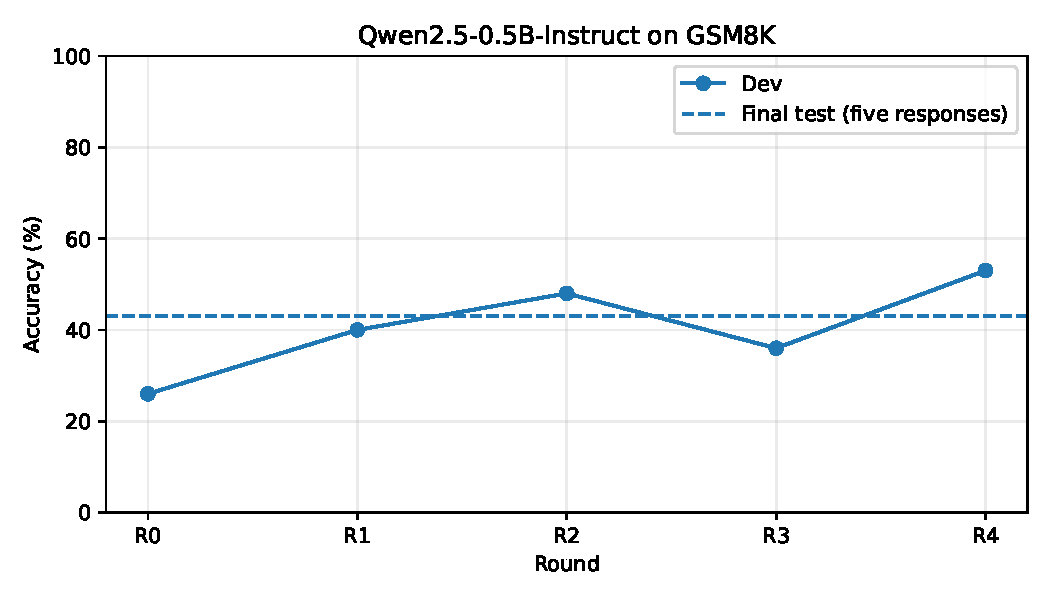
\includegraphics[width=.72\linewidth]{rsi_curve.pdf}
\caption{Dev accuracy across rounds. The dashed line marks the test score of the final five-response configuration. R4 uses the R2 prompt.}
\end{figure}
R1 corrected 18 R0 errors and introduced four, raising dev accuracy from
26\% to 40\%. The token-limit rate fell from 70\% to 29\%.
Although R1 produced fewer output tokens, it took longer to run
(66.5 versus 56.3 seconds); its prompts also included two worked examples.

In the R2 search, R0 and R1 scored 15\% and 25\% on the 20-question subset.
The eight proposals scored 45, 35, 30, 30, 45, 45, 25, and 40\%.
The first proposal remained selected and scored 48\% on the full dev set,
correcting 18 R1 errors and introducing ten.

R3 corrected nine R2 errors but introduced 21, reducing accuracy to 36\%.
Its answer-marker rate rose to 34\% and its token-limit rate fell to 14\%:
better output formatting coincided with more incorrect answers.
R4 used the R2 prompt and corrected ten of its errors while introducing five,
reaching 53\%. Forty-seven questions triggered two extra responses, for
394 generations in total. R4 used 4.36 times R2's output tokens and
3.39 times its inference time.
\begin{table}[H]\centering\small
\begin{tabular}{lrrr}
\toprule R1 component & Dev & Cap rate & Output tokens \\
\midrule
Neither (R0) & 26\% & 70\% & 24,488 \\
Instruction only & 37\% & 44\% & 22,360 \\
Demonstrations only & 48\% & 31\% & 19,893 \\
Both (R1) & 40\% & 29\% & 17,510 \\
\bottomrule\end{tabular}
\caption{Instruction and demonstration ablation; all other settings are fixed.}
\end{table}
\begin{table}[H]\centering\small
\begin{tabular}{lrrrr}
\toprule Decoding & Dev & Generations & Output tokens & Seconds \\
\midrule
Greedy (R2) & 48\% & 100 & 15,098 & 61.6 \\
Fixed three & 49\% & 300 & 48,949 & 173.8 \\
Adaptive (R4) & 53\% & 394 & 65,839 & 208.5 \\
Fixed five & 56\% & 500 & 82,447 & 276.1 \\
\bottomrule\end{tabular}
\caption{Sampling comparison with the same R2 instruction and static demonstrations. All sampled variants include one greedy answer.}
\end{table}

\section{Analysis and Conclusion}
\subsection{How the answers changed}
Case IDs below refer to indices in the original training split.

\paragraph{R1: shorter responses, persistent arithmetic errors.}
In ID 5878, the correct cost was $6(0.25)+3(0.5)+2(2)=7$ dollars.
R0 reached the token limit with an extracted answer of 4. R1 finished the
calculation but wrote $1.5+1.5+4=6.5$.
All five cases used to design R1 remained incorrect. Its gains came from
other questions: for example, ID 5710 required $(5000-2900)/700=3$ months,
and the prediction changed from 12 to 3.

\paragraph{R2: identifying the requested quantity.}
In ID 2437, an account started at \$100 and spent \$8 per day for seven days,
leaving \$44. Withdrawing as many \$5 bills as possible left \$4.
R1 computed the remainder but returned \texttt{\#\#\#\# 40}, confusing
the withdrawn amount with the amount left. This error was included in
the improver's feedback. Under the R2 prompt, the response ended with
\texttt{44 - 40 = 4} and \texttt{\#\#\#\# 4}.

\paragraph{R3: relevant vocabulary, incorrect operations.}
ID 4632 asked for each waiter's share of a 20\% tip on meals costing
\$10, \$20, and \$30. The answer was $(10+20+30)0.2/3=4$.
R2 predicted 10. R3 retrieved demonstrations 11, 6, and 10, including a
percentage/tax example, yet predicted 20.
In ID 819, the remaining 200 tins had to be collected over four days,
giving an answer of 50. R2 predicted 200; R3 retrieved time-related examples
and predicted 40. The retrieved examples matched parts of the vocabulary
without resolving the operation errors.

\paragraph{R4: recovery through sampling and early stopping on errors.}
For ID 819, R4 produced the parsed answers $[200,40,69.4,50,50]$.
The first three disagreed, and the additional pair made 50 the most frequent
answer. In ID 3115, removing one quarter of 572 beans left 429;
removing a third of those left 286; half of the remainder was 143.
R2 predicted 71, and R4 produced $[71,71,242]$. The repeated wrong answer
triggered early stopping. These cases show how the same agreement rule
can recover an error or preserve it.

\subsection{Ablations and inference cost}
The R1 ablation separated the effects of instructions and demonstrations.
Accuracy was 26\% with neither change, 37\% with the revised instruction,
48\% with demonstrations, and 40\% with both. Adding the revised instruction
to the demonstration prompt reduced accuracy by eight points, while reducing
the token-limit rate from 31\% to 29\%. The combined prompt produced shorter
answers and scored lower than the demonstration-only prompt.

Three responses per question yielded 49\% dev accuracy, adaptive sampling 53\%, and five responses 56\%. Compared with five responses, adaptive sampling used 21.2\% fewer generations and 20.1\% fewer output tokens, at 3 percentage points lower accuracy. The five-response configuration was selected for its higher dev accuracy. 
Adaptive sampling generated its extra responses for a subset of questions,
whereas the five-response variant generated them for all questions.
The different batch shapes changed random-number consumption, so the fourth
and fifth responses were not paired across the two variants. Their measured
difference combines the stopping rule with sampling variation.

Target-model generation across all recorded stages took \LocalMinutes{}
minutes, excluding model loading, downloads, and API waiting.
The eight improver calls used 39,118 input tokens and 597 output tokens;
a separate connection check used 43 tokens.

\subsection{Generalization and conclusion}
The selected configuration scored \FinalDev{} on dev and \FinalTest{} on
test. Development-set selection and variation between the question samples
are plausible contributors to the \FinalGap{}-point gap.
The experiment used one seed, 100 questions per evaluation split, and a
20-question search subset. Each test answer therefore changed accuracy by
one percentage point. Repeating the comparison across larger splits and
multiple seeds would give a clearer estimate of the gains.

For this model and demonstration pool, improving the static prompt was more
effective than retrieving examples by lexical similarity. Additional samples
raised dev accuracy further, with the five-response variant reaching 56\%.
Adaptive sampling reduced generation cost by about one fifth, at a cost of
three accuracy points. The bean-counting example shows how early agreement
can preserve a shared mistake.

\begin{thebibliography}{9}
\bibitem[CUHK-Shenzhen(2026)]{course} CUHK-Shenzhen NLP Course. 2026.
Assignment 3 and the \emph{Track C prompt optimization reference notebook}.
\bibitem[Qwen Team(2024)]{qwen} Qwen Team. 2024.
\emph{Qwen2.5-0.5B-Instruct model card}.
\url{https://huggingface.co/Qwen/Qwen2.5-0.5B-Instruct}.
\bibitem[DeepSeek(2026)]{deepseek} DeepSeek. 2026.
\emph{API documentation: Your First API Call; Thinking Mode}.
Accessed November 23, 2026. \url{https://api-docs.deepseek.com/}.
\bibitem[Wang et al.(2023)]{wang} Xuezhi Wang, Jason Wei, Dale Schuurmans,
Quoc Le, Ed Chi, Sharan Narang, Aakanksha Chowdhery, and Denny Zhou. 2023.
Self-Consistency Improves Chain of Thought Reasoning in Language Models.
\emph{ICLR}. \url{https://arxiv.org/abs/2203.11171}.
\end{thebibliography}
\end{document}
